% !TEX encoding = UTF-8 Unicode
\documentclass[a4paper,10pt]{article}
\usepackage[utf8]{inputenc}
\usepackage{listings}
\usepackage[francais]{babel}
\usepackage[T1]{fontenc}
\usepackage{graphicx}

\author{Présent: Tous (sauf Jérome, excusé par son impossibilité de venir)}
\title{PV réunion 4}
\date{13 décembre 2013}

\begin{document}
\maketitle
\Large (Version pré-finale)
\part*{Changement diagrammes UML}
\begin{description}
\item[\Large Diagramme de séquences] :\\
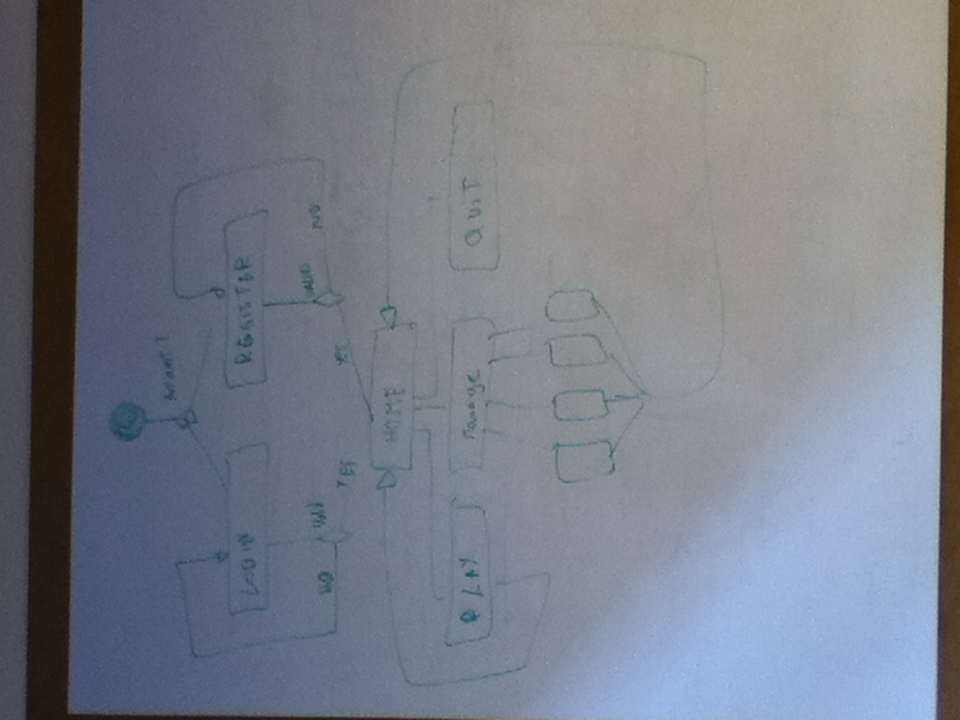
\includegraphics[angle=-90, scale=0.5]{Sequence_Diagram.JPG}
\newpage

\item[\Large Diagramme d'utilisation] :\\
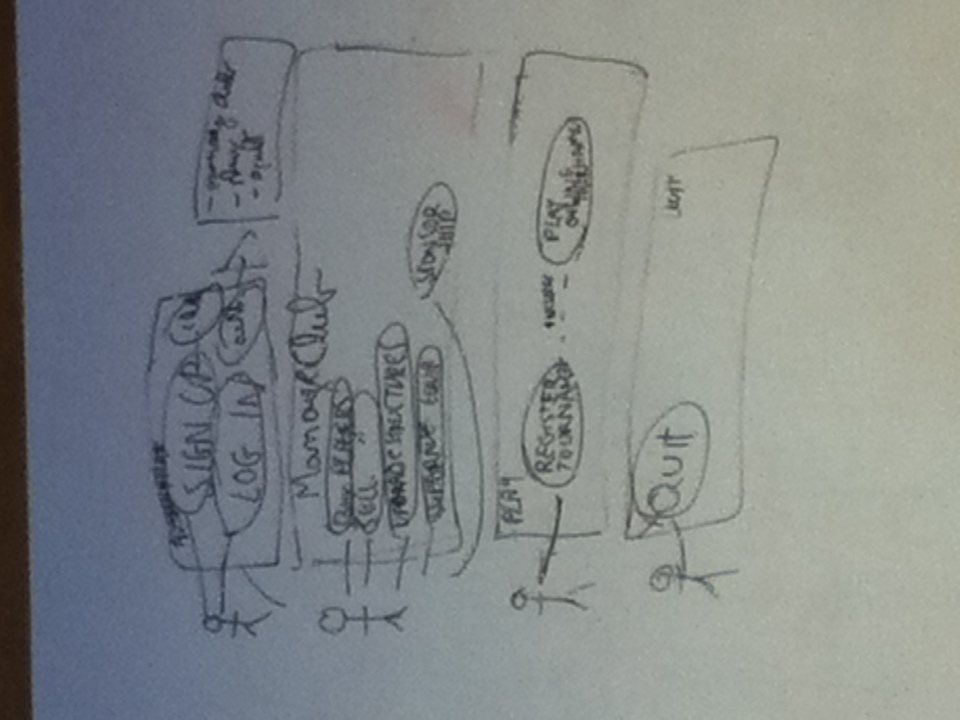
\includegraphics[angle=-90, scale=0.5]{Use_Case_Diagram.JPG}
\newpage

\item[Diagramme de classes] :\\
Discussion pour enlever la classe team : Elle sert seulement de conteneur et n'a pas de sens telle qu'elle est actuellement\\=> remplacer par deux listes arguments de club, nonFieldPlayers et team, qui pointent vers des objets nonFieldPlayer, team devant en contenir toujours 7, et nonFieldPlayer contenant l'ensemble des joueurs disponibles au club\\ /!\textbackslash{} problème, pas de représentation en UML (?)

Rappel sur le fait que les nonFieldPlayer doivent être cast en fieldPlayer lors de l'entrée en match, en faisant attention à ne pas prendre d'information (permet d'éviter un surplus de méthodes(?) non utilisée dans un cas ou l'autre)
\end{description}
\part*{Communication et outil}
\begin{description}
\item[Communication] : IRC (freenode\#aucuneidee)
\item[Outil UML] : Remplacement de argoUML par Umbrello (par praticité)
\end{description}
\end{document}